\section{Robust Motion Isolation} 
\label{sec:motion}

As discussed previously, our Gaussian mixture model does an excellent job of
distinguishing traces of moving objects from traces of static objects caused
only by the motion of the camera.  We decided to apply this aspect of our model
to the task of isolating motion in a scene, regardless of unstable video
footage.  We first describe the model we use to take traces and corresponding
GMM probabilities and create a video with only the moving elements.  We then
describe the experiments and results of our implementation.

\subsection{Model Application} % (fold)
\label{sub:Model Application}

\paragraph{Traces to Frames} % (fold)
\label{par:Traces to Frames}

Our problem can be formulated as follows: Given a set of traces and the GMM
probability for each, we look to find the probability that pixel $\pi_j =
(x_j,y_j)$ at time $t$ is of a moving object in the scene or not.  In order to
calculate this we first transform a few parameters.  First, we invert and bound
the range of GMM probabilities to create a movement score.  Given ${\bf
P}$ is the vector of log-probabilities returned by the GMM for a given set of
traces, we create the following vector of movement scores:
\begin{align}
	{\bf s} = - \frac{ {\bf P} - {\rm max}({\bf P}) }{ {\rm min}({\bf P}) }
\end{align}
Under this transformation, the scores are monotonically bound to the range $[0,1]$, with
more likely moving objects (trace differential outliers) closer to 1. 

With this score, we can create a probabilistic model for any given pixel representing
 a moving object or not.  In our model we assume independence among both
pixels and traces.  Therefore, given score $s_i$ for trace $T_i$, at position
$(x_{i,t},y_{i,t})$ at time $t$, we claim the following probabilities:
\begin{align}
	P(s_i,x_{i,t},y_{i,t}|{\rm pixel}_j = {\it moving})  &= \frac{1}{1 + e^{-\gamma(s_i - \beta)}} e^{- \frac{|(x_{i,t},y_{i,t}) - \pi_j|^2}{\alpha_1}}
	\\ P(s_i,x_{i,t},y_{i,t}|{\rm pixel}_j = {\it static})  &= \left( 1 - \frac{1}{1 + e^{-\gamma(s_i - \beta)}}\right) e^{- \frac{|(x_{i,t},y_{i,t}) - \pi_j|^2}{\alpha_2}}
\end{align}
The first term in each probability puts the movement score through the logistic
function in order to partition scores into being generally very close to zero
(most likely static) or very close to one (most likely moving).  For this
logistic function we have two parameters: $\beta$ and $\gamma$.  $\beta$ we
pick as some threshold score for which scores less than the threshold are
pushed to 0 and scores greater than the threshold are pushed to one.  Picking
this threshold is similar to the problem of picking the threshold for the
structure for motion problem.  While this could be done dynamically based on an
analysis of the score distribution, similar to that in Figure
\ref{fig:logpdfs}, we generally used a threshold at about the 75th percentile
mark to separate the scores.  (Remember that scores are inverted such that high
scores are more likely to be of moving objects.)  The parameter $\gamma$ is
used to push values toward zero or one and leave few values near 0.5; we set
$\gamma = 100$.

The second term encodes Gaussian-falloff based on the distance between
each feature and pixel to determine what influence that feature's score has
on the probability for that pixel.  The terms $\alpha_1$ and $\alpha_2$
determine the width of the Gaussian.  With this function we make sure
that features closer to a pixel have a stronger influence on their probability
than pixels far away.  Based on experimentation, we set $\alpha_1 =
2\alpha_2$ so that features that appear to be moving having a wider range of
influence than those that do not.


Given these probabilities for trace scores conditional on pixel movements, we
can calculate the general probability of a pixel being of a moving or static
object, following Bayes rule
\begin{align}
	P({\rm pixel}_j = o|{\bf s},W) = \frac{ P({\bf s},W|{\rm pixel}_j = o) P({\rm pixel}_j = o) }{ P({\bf s}, W) },
\end{align}
where $o \in \{ {\it moving}, {\it static} \}$.  We make the assumption that we
have no priors on pixels nor traces.  Also, because under our model we assume
independence among traces, we can simplify our calculation to the following equation
\begin{align}
	\log P({\rm pixel}_j = o|{\bf s},W) = \sum_i \log P(s_i,x_{i,t},y_{i,t}|{\rm pixel}_j = o) \label{eq:logsum}
\end{align}
At the end of the calculation, if $P({\rm pixel}_j = {\it moving}|{\bf s},W) > P({\rm
pixel}_j = {\it static}|{\bf s},W)$ then we consider the pixel to be of a moving object,
and if not we consider it to be static.  Doing this for all pixels in each
frame, we can construct a video isolating only the moving elements.

% paragraph Traces to Frames (end)

\paragraph{Trace Sets} % (fold)
\label{par:Trace Sets}

One key challenge in performing feature tracking is that features
are often lost if tracked over many frames.  In the case of motion
isolation, we do not care if any given feature is tracked continuously,
but rather just if each pixel is more likely to be of a moving or static
object.


\newcommand{\fset}{ \EuScript{F} }
\newcommand{\fstep}{ f_s }
\newcommand{\fwin}{ f_w }

%\nico{yeah, this paragraph below could use work, but I'm not sure how to fix it specifically }

Therefore, to minimize feature loss and to otherwise encourage more tracked
features per frame, we break the video into shorter sets of frame, each frame set denoted by
$\fset_k$.  In order to keep some of the elements of tracking across the video,
we have some overlap between frame sets, which we denote as frame step
$\fstep$.  Therefore, the first frame of $\fset_k$ is $\fstep$ frames after the
first frame of $\fset_{k-1}$. Frame sets have a window size $\fwin$, such that
they contain a total of $\fwin\fstep$ frames, or alternatively, each frame is
part of $\fwin$ frame sets.
(In practice we set $\fwin = 3$ and $\fstep = 3$ or 5.)

Given such a set up, we can run our previously described algorithm, calculating
the GMM, movement scores, and pixel movement probabilities for each frame set.
Because we assume independence among traces, we can simply include the
log-probabilities for each frame set together in the sum in Equation
\eqref{eq:logsum}, leaving us still with the final comparison $P({\rm pixel}_j
= {\it moving}|{\bf s},W) > P({\rm pixel}_j = {\it static}|{\bf s},W)$ to
determine if a pixel is more likely to be of a moving object or not.

% paragraph Trace Sets (end)



% subsection Model Application (end)

\subsection{Experiments} % (fold)
\label{sub:Experiments}


\paragraph{Setup} % (fold)
Our implementation followed the algorithm given above fairly closely, and only
required adjusting parameters slightly depending on some unique video features
like image resolution.  As there was no simple ground truth, we largely
evaluated our results based on the quality of the movie produced.  We ran our
algorithm on a number of different data sets: two videos collected with the Samsung
mobile phone of the authors walking around a computer lab and two
low quality home-videos downloaded from YouTube.  We ran our algorithm over a 
selected portion of each video.  In each frame,
pixels that were more likely to be of static objects than moving objects were
removed, leaving only the ``moving pixels.''  The results are discussed below.

% paragraph Setup (end)

\paragraph{Results} % (fold)
\label{par:Results}

Overall, the algorithm ran as desired.  In each video we generally isolate the
parts of the scene that are moving.  Figure \ref{fig:alex-walking} gives an
example of the steps of the process for a video of Alex walking through the
lab.  The video generally captures where he is and removes the
background.

\begin{figure}[tb]
	\centering
	\begin{subfigure}[b]{0.33\textwidth}
		\centering
		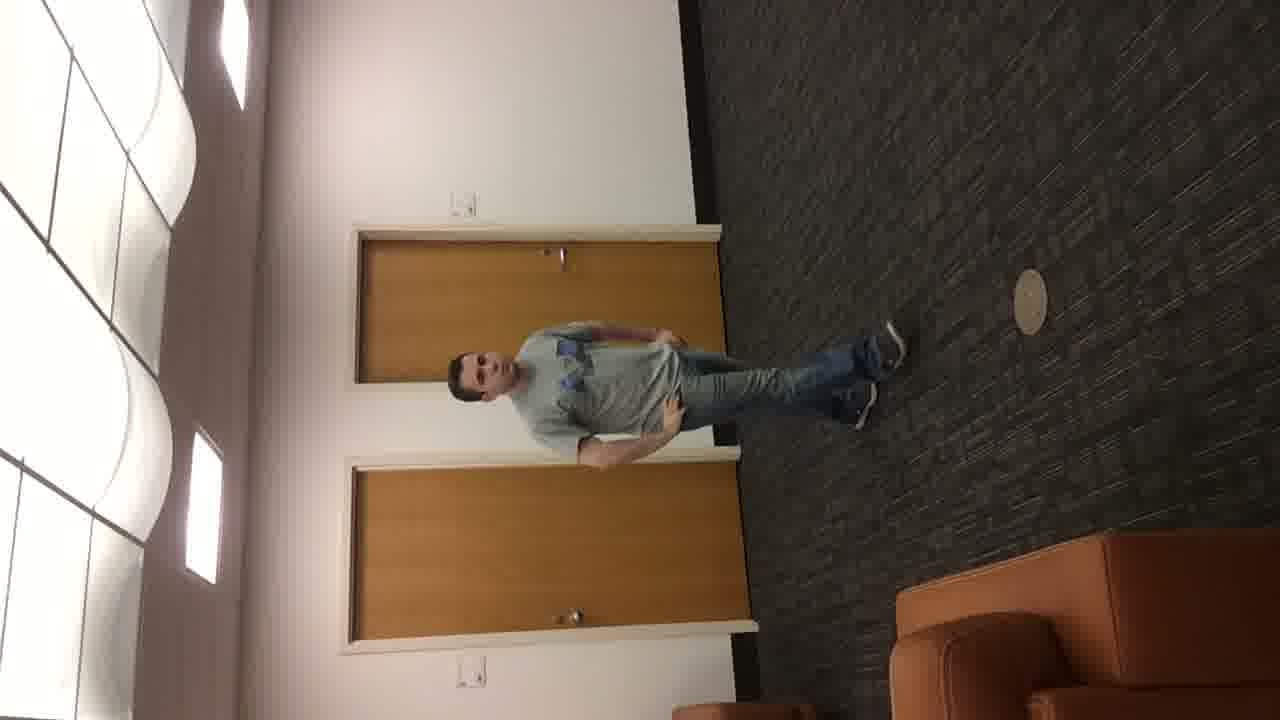
\includegraphics[width=2.9in,angle=-90]{figs/alex-image30.jpg}
		\caption{Single frame before analysis.}
	\end{subfigure}%
	\begin{subfigure}[b]{0.33\textwidth}
		\centering
		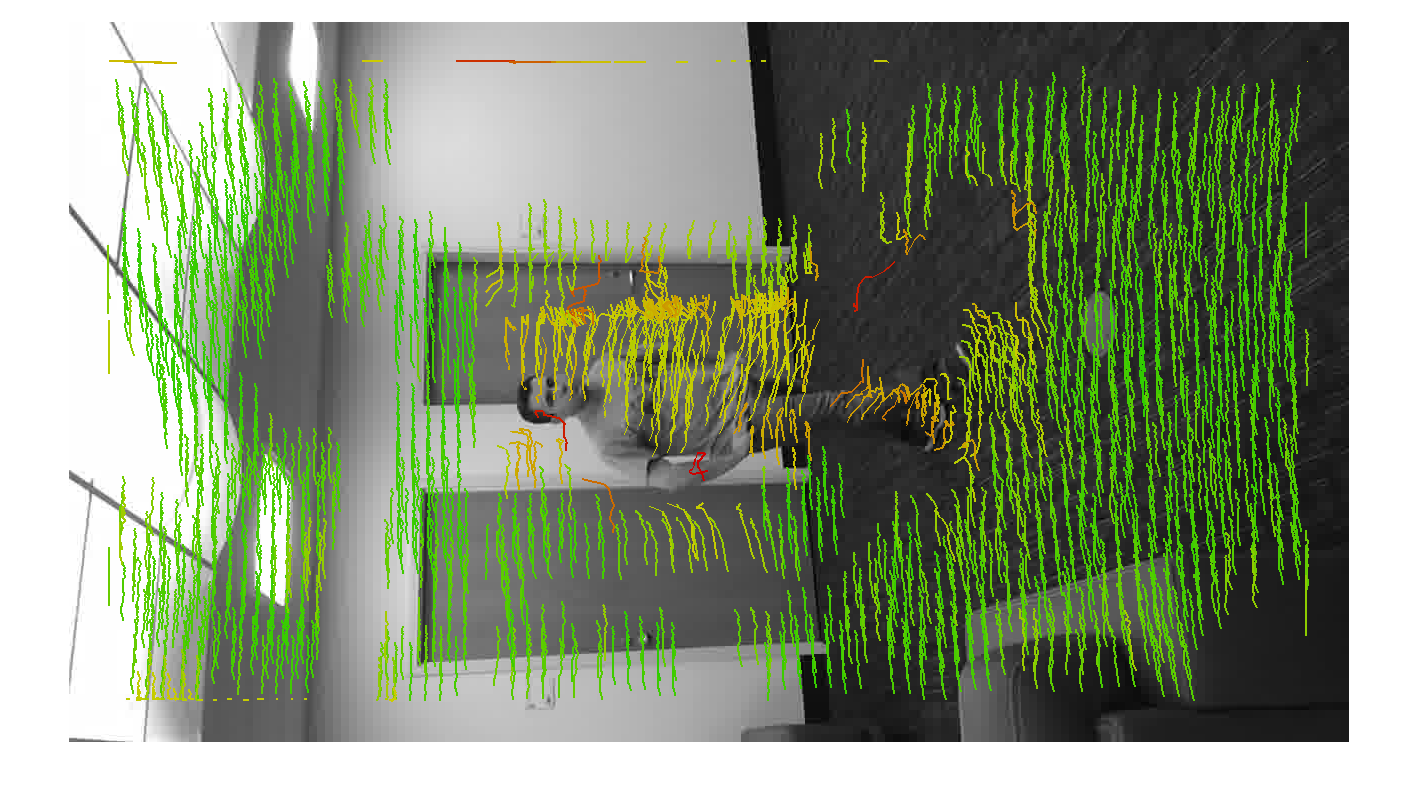
\includegraphics[width=3.1in,angle=-90]{figs/gmm-motion.png}
		\caption{Traces with by GMM probability}
	\end{subfigure}%
	\begin{subfigure}[b]{0.33\textwidth}
		\centering
		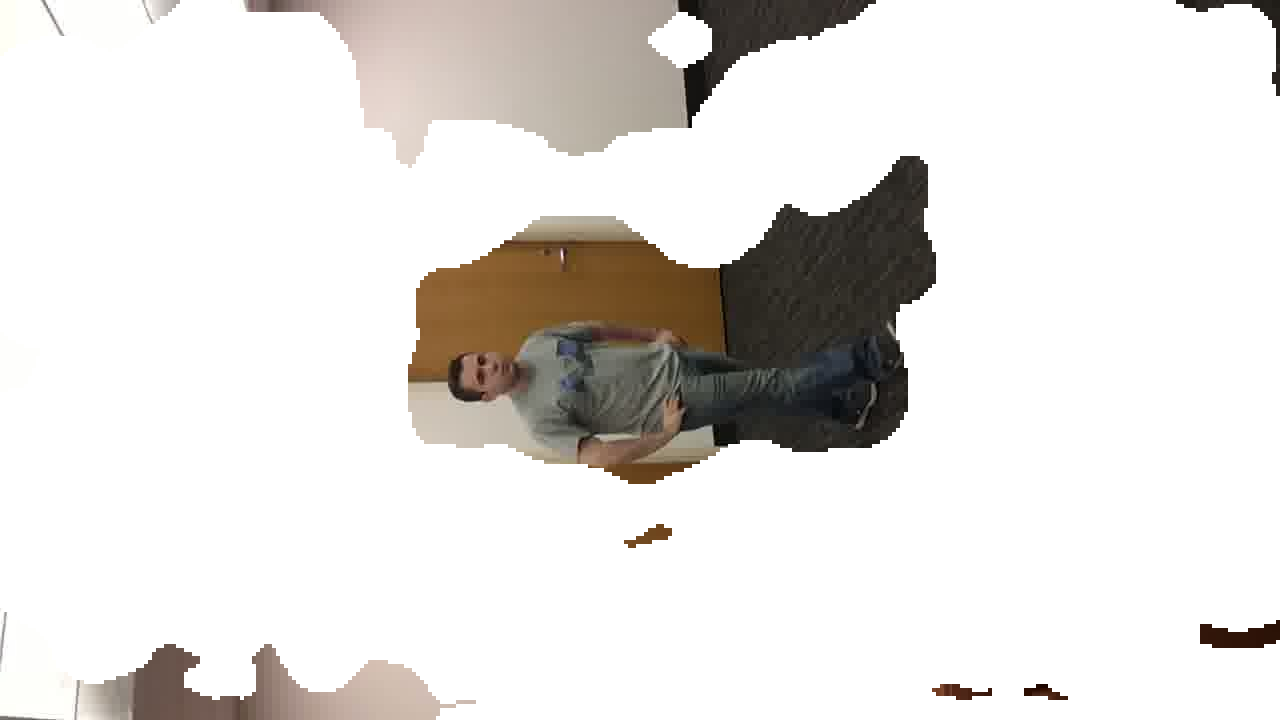
\includegraphics[width=2.9in,angle=-90]{figs/alex30.png}
		\caption{Frame after motion isolation}
	\end{subfigure}%

	\caption{Step through of our algorithm running on video we took of Alex walking.}
	\label{fig:alex-walking}
\end{figure}

In practice we found that videos of dancing were excellent examples as the
motion of the person was very distinct from the motion of the
background.  On YouTube we found two famous videos of dancing: ``Bimbo Dancer''
\cite{bimbodance} and ``Break Dance Kick'' \cite{breakdance}.  Both videos are
relatively low quality with a shaky camera, but our algorithm performs well.
In Figure \ref{fig:bimbodance} we see a baby dancing on a table, and the
algorithm successfully picks out his traces as unique from those in the
background.

\begin{figure}[tb]
	\centering
	\begin{subfigure}[b]{0.33\textwidth}
		\centering
		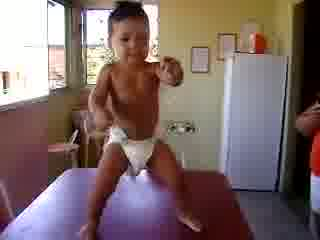
\includegraphics[width=0.9\textwidth]{figs/bimbodance-image50.jpg}
		\caption{Single frame before analysis.}
	\end{subfigure}%
	\begin{subfigure}[b]{0.33\textwidth}
		\centering
		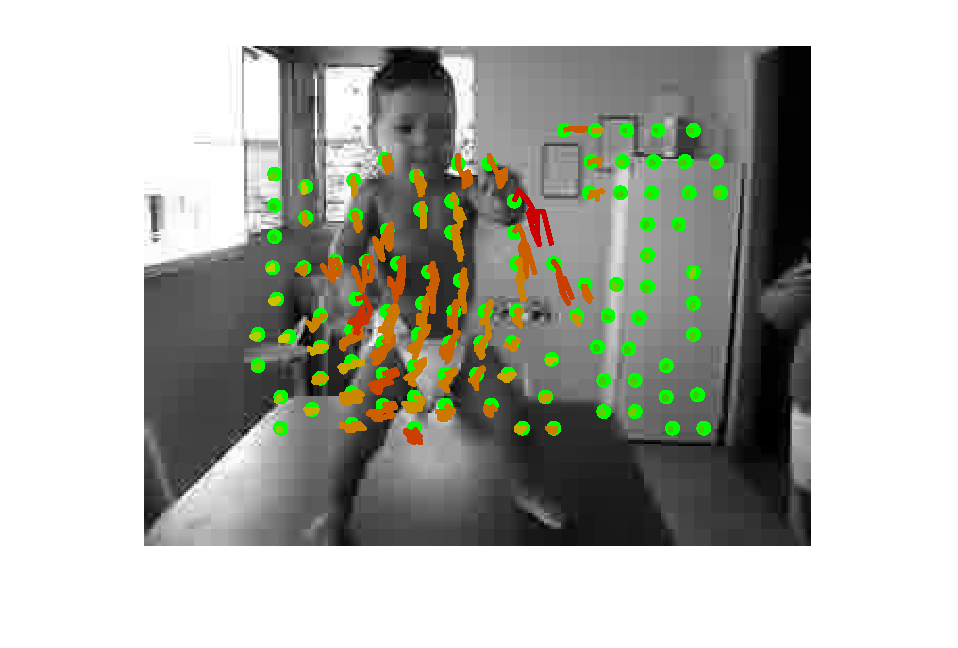
\includegraphics[width=1.1\textwidth]{figs/bimbodance-50.pdf}
		\caption{Traces with by GMM probability}
	\end{subfigure}%
	\begin{subfigure}[b]{0.33\textwidth}
		\centering
		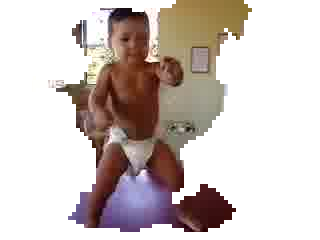
\includegraphics[width=0.9\textwidth]{figs/bimbodance-image50.png}
		\caption{Frame after motion isolation}
	\end{subfigure}%

	\caption{Step through of our algorithm running on video of a baby dancing \cite{bimbodance}.}
	\label{fig:bimbodance}
\end{figure}

Complete videos of the output can be found online at \url{http://alexbeutel.com/10701/motion.html}.
Overall we were pleased with the result, though we believe fine-tuning the
parameters of the model could improve the output.  We also believe that
combining this information with computer vision techniques, such as image
segmentation, could produce much more robust results.


% YouTube Videos:
% http://www.youtube.com/watch?v=6LOj0_Ufemc
% http://www.youtube.com/watch?v=sCM4dREGdDw

% paragraph Results (end)



% subsection Experiments (end)
